\documentclass[a4paper,11pt]{article}

\usepackage{float}
\usepackage{graphicx}
\graphicspath{./Diagrams}

\setlength{\oddsidemargin}{0in}
\setlength{\evensidemargin}{0in}
\setlength{\textwidth}{160mm}
\setlength{\topmargin}{-15mm}
\setlength{\textheight}{240mm}



\title{Applying AI to Solve a Single Player Puzzle Game(Solitaire)}

\author{Sam David Freeman}


\begin{document}

\begin{center}
	\textbf{{\Large Applying AI to Solve a Single Player Puzzle Game(Solitaire)}}
\end{center}
\begin{center}
	Author: Sam David Freeman (sdf2@aber.ac.uk)
\end{center}
\begin{center}
	Supervisor: Dr Thomas Jansen (thj@aber.ac.uk)
\end{center} 
\begin{center}
	G400 Computer Science BSc
\end{center}
\begin{center}
	CS39440 Major Project
\end{center}
\begin{center}
	25th April 2023
\end{center}
\begin{center}
	Draft 1.0
\end{center}
\newpage




\section*{\centering Declaration of originality}

I confirm that:

\begin{itemize}
	\item{This submission is my own work, except where 
		clearly indicated.}
	
	\item{I understand that there are severe penalties for Unacceptable Academic Practice, which can lead to loss of marks or even the withholding of a degree.}
	
	\item{I have read the regulations on Unacceptable Academic Practice from the University's Academic Registry (AR) and the relevant sections of the current Student Handbook of the Department of Computer Science.}
	
	\item{In submitting this work I understand and agree to abide by the University's regulations governing these issues.}
\end{itemize}

\vspace{2em}
Name: Sam David Freeman  \\

\vspace{1em}
Date: 05/05/2023 \\
\newpage

\vspace{1em}
\section*{\centering Consent to share this work}

By including my name below, I hereby agree to this project's report and technical work being made available to other students and academic staff of the Aberystwyth Computer Science Department.  

\vspace{2em}
Name: Sam David Freeman  \\

\vspace{1em}
Date: 25/04/2023 \\
\newpage
\section*{\centering Acknowledgements}

I am grateful to...

I'd like to thank...
\newpage
\section*{\centering Abstract}

\newpage
\tableofcontents
\newpage
\section{Background}
	
\subsection{Problem description}
The logic based combinatorial number placement puzzle Sudoku, is a well-established puzzle game which grew popular in Japan in the 1980s. The classic game of Sudoku consists of a 9x9 grid of spaces, which can only be filled with numbers between 1 and 9. Each space in the 3x3 block, vertical and horizontal columns can only have each number between 1 and 9 once. The puzzle is completed when all spaces in the grid have been filled and no earlier rule has been violated. A more generic description of the puzzle, describes a grid of NxN in size, with N grids contained, using numbers between 1-N. [Add reference to https://sudoku.com/sudoku-rules/]
\subsection{Background}
Sudoku is a well established and solved puzzle, with a proven efficient way to be solved established. However, there are other admittedly less efficient AI methods which can be applied to solve this and provides an interesting way to apply and experiment with AI methods learnt at university to a real problem.\newline \newline
Peter Norvig solved Sudoku [Add reference here https://norvig.com/sudoku.html], using both constraint propagation and search, so the most efficient method is too established. However, looking at a book[ add reference to A modern approach], using a different heuristic search approach seems to be a better way, which has been used before but not fully explored was in there. \newline \newline
Using evolutionary algorithms(EA), specifically based off the Russel/Norvig approach [modern approach reference] to solve seems like an interesting and most importantly different way to solve the problem, which can also solve several different size puzzles with some level of efficiency. Equally a normal evolutionary algorithm on its own will need some help to be able to solve the sudoku at all leaving several different options, this includes using different hybrid methods to add constraints to the problem, or having constraints included as part of the evolutionary algorithms fitness function.\newline\newline
EA has several terms that will be used throughout this report.\\
\begin{itemize}
	\item Population - The total number of individuals in the algorithm
	\item Individual - Each state used to represent the objects the algorithm is solving
	\item Fitness function - A function used to rate each individual in the population based on viable a solution it is
	\item Selection - The process of taking only a section of the population based on their fitness
	\item Crossover - The process of mixing parts of the individuals to produce new variation children 
	\item Mutation -  The process of randomly changing a gene within individuals
	\item Multi-objective EA - Where the fitness function uses more than one numerical value to rate each individual
\end{itemize}
\subsection{Analysis}
The evolutionary algorithm will need a few key items at implementation:
\begin{itemize}
	\item A way to encode the puzzle
	\item A fitness function
	\item A selection process for the population
	\item A mutation function
\end{itemize}
For the fitness function there are two different ways it can be done, a simple fitness function which does not enforce the rules of sudoku, this would need a hybrid approach to help enforce the rules. Alternatively, a more complex fitness function, that considers several factors, to look at fitness i.e., a multi-objective evolutionary algorithm.\newline \newline
For solving the sudoku a hybrid evolutionary algorithm, there are several different hybrid approaches existing []. The recommended approach for a constraint optimization problem such as sudoku is a repair method. The repair method would work to enforce the rules of the puzzle, by changing each individual in the population that violates the constraints bringing it back into the range of viable solutions.\newline \newline
These two different methods both have valid ways of solving the Sudoku and create a new question. Does a hybrid approach using a repair method work better than a classical approach using multi-objective EAs? They can be compared on, number of generations, runtime, number of puzzles stuck on and looks at patterns between different sudoku puzzle difficulties and seeing if the pattern of human difficulty has any relationship to how long it takes for each EA to solve the puzzle.

\subsection{Process}
The lifecycle model used in this project, takes the most helpful aspects of different life-cycles, and applies them to be of the most use in this project. The most important and closely followed part of the process is the use of the Kanban board, used to keep track of what tasks there were to do. From Scrum the ideas of sprints and stories are used to build up a log of tasks which are used on the Kanban board and a weekly meeting which were used to review what work had been done that week, discuss improvements on that work and talk about targets for the next week.\newline \newline However, the underlying process used in project is closer to waterfall, with the requirements and research being done first, followed up by implementation, testing and maintenance. Overall, it would describe the process as waterfall with different agile aspects.


\section{Experiment methods}

\subsection{Experiment 1}
There are two distinct algorithms being used in this project, the Hybrid Repair and the Multi-objective algorithm. These two algorithms both have there strengths and weaknesses and whilst not the ideal choice for solving sudoku, one of these methods might be better than the other. So the question becomes: 
\begin{itemize} 
	\item How does a hybrid repair EA algorithm compare to a Multi-objective EA? 
	\item Is one method more efficient than the other?
	\item Is one method more consistent than the other?
	\item Is there a large difference in runtime?
\end{itemize}
The first question can be answered by looking at the next three questions. For finding out the efficiency or effectiveness of the algorithms, looking at and comparing the number of generations it takes to get to the solution.  For finding out the consistency of the algorithms, looking at the number of times each algorithm fails to solve the puzzle it is presented and also looking at the standard deviation from the average number of generations and runtime. \newline \newline The final question has the least impact on the overall investigation, as it can be affected the most by outside factors, however looking at the average runtimes and standard deviations from the average can clearly show how fast each algorithm generally, however it also worth noting, that this could be due to inefficient programming rather than the algorithms design itself. Due to the randomness of both of the algorithms, both sets of results will have to process and compared using a statistical test which can data that is not normally distributed such as a Wilcoxon test.
\subsection{Experiment 2}
The second and arguably more interesting question being looked at in this project, concerns difficulty in Sudoku puzzles. With Sudoku puzzles, there are two main ways to increase the difficulty of the puzzles, the first is by increasing the size of the puzzle, as with larger puzzles, there are more numbers involved and more potential solutions. Meaning that inherently a 4x4 puzzle is easier than a 9x9 puzzle. The other way in which difficulty can be measured for people, is by changing the number of initial squares that are filled. Concerning the minimum number of spaces required for a unique solution to be found by a human, research has been done and it has been found that a minimum of 17 filled in spaces are needed for a Sudoku to be solvable.\newline \newline For the purposes of this question broader catagories for difficulty, will be more appropriate, this will be done by using sudoku generated by Sudoku.com[] and using their difficulty system of Easy, Medium, Hard and Extreme puzzles. The interesting part comes from looking for a link between the difficulty that humans find solving these puzzles and the algorithms that are designed to do so. By looking at both algorithms and using them on different difficulty sets, some questions are created:
\begin{itemize}
	\item Is there a correlation between human difficulty and algorithm performance?
	\item Does either algorithm perform particularly well with a certain difficulty or size puzzle? Why?
	\item Is there a relationship between initial puzzle size and generations?
\end{itemize}
For the first question, looking at a mapped graph displaying difficulty against runtime and generations. For the second question, looking at the results for the datasets on both sides for each difficulty and finding any noticable difference in the averages outside of the conclusions from experiment 1. The final question further builds on question 1, by seeing if the correlation is simply due to the size of the puzzle given.

\subsection{Approach for Hybrid Repair method}

The idea for the hybrid method is, firstly much like a normal EA the population of the puzzle is created , this will be generated from many starting mutations on the initial sudoku puzzle given. The next step is a loop, that if there are no violations and no empty spaces in any puzzle population, or alternatively the algorithm has reached the maximum number of generations, ends the loop and returns the solution if there is one, otherwise the rest of the steps are taken, all of which are contained within this loop. The next step is sorting and selection, this will take the population, sort them based on their fitness values and then removes half the puzzles from the population. The remaining members of the population would then mutate, creating a mutated child, pushing the population back to the intended size and mutating itself. After this the repair algorithm, looks at every member of the population that is currently breaking one of the games rules and brings it back into the range of a feasible solution. The final step is updating the fitness values of the population, and then loops back to the decision.
\begin{figure}[h]
	\caption{Flow diagram for Hybrid repair method}
	\centering
	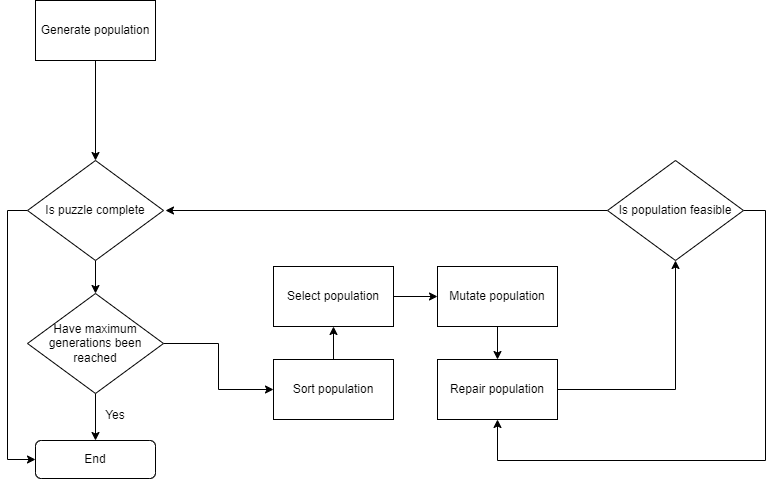
\includegraphics[height=8cm, width=15cm]{./Diagrams/hybridRepairFlowchart}
\end{figure}
\subsection{Approach for Multi-objective method}
The idea for the multi-objective method starts the same as the hybrid method, with generating the population of the puzzle. The next step is once again the same as for the hybrid repair method, the loop which ends if there are no violations and no empty spaces left in the puzzle or the maximum number of generations, and returns the solution if one was found. The next step is then mutating the puzzle, which in this algorithm, creates a copy set of children from the full population, mutates the children and then updates the fitness value of the children. The selection function now creates a new population, which is made from a combination of the two old populations, with the best between each parent and child pair being added to the new population.  

\begin{figure}[h]
	\caption{Flow diagram for Multi-objective method}
	\centering
	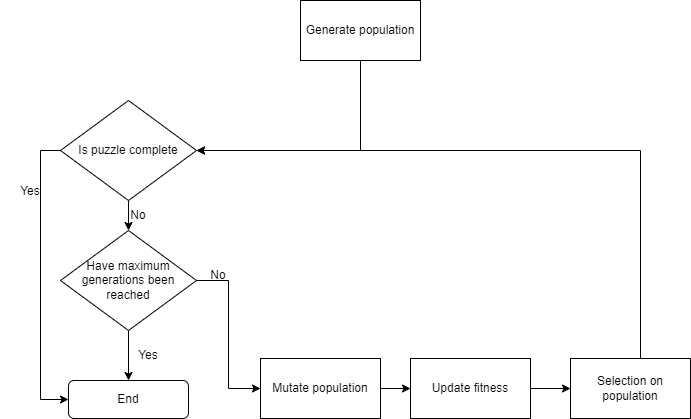
\includegraphics[height=8cm,width=15cm]{./Diagrams/multiobjectiveFlowchart}
\end{figure}

\subsection{Experiment design}

The experiment, program will go over a set of 10 puzzles in a folder. For each puzzle in the dataset, it will loop through and solve each program storing the generations and time taken for each puzzle in an output file specific for that puzzle. Once all 30 runs of the solver have been done, the averages for the program can be calculated, the averages will not include failed attempts, as this will massively change the results and averages for successful runs. The failures will also be calculated and with the averages be added to a file specific to the puzzle size and difficulty. These results can then be processed using R, to create more meaningful data.

\subsection{Tools}
The programs used in this project are coded in Java 18, and are written in the IntelliJ IDEA IDE development environment. This is due to familiarity with the language and development environment. Within the development the use 3rd party library through Maven, JUnit was needed, to test individual features and functions of certain key methods, including ones listed in the requirements(see Chapter 3.1). GitHub was used as a version control tool and also used for project management , this was necessary as it allowed for a backup file system, which can be added to from different places, as well as providing a feature which can be used as a kanban board(mentioned in 1.4).
The statistical analysis needed for the experiments use the programming language R to perform the tests and produce graphs based on the data produced. texStudio and LaTeX were used in the creation of documentation providing a way to structure and document the final report for the project. The diagrams used in the documentation, were created using the tool draw.io, created diagrams visually explaining concepts, flowcharts used to show the basic outline of the program and class diagrams detailing each part of the project. 


\section{Design}
For the overall design of for the solver experiment code can be split into, the solving algorithms, and the sudoku puzzles representation. There will be two different versions of the solver, which have common features, can use object oriented principle of inheritance which will also help at the later on stages of the experiment code, using polymorphism. The collection of puzzles(population) will also be an attribute in the solver class.

\subsection{Requirements}

Load sudoku puzzles from a file\newline
For the Hybrid repair algorithm:
\begin{itemize}
	\item Solve a 4x4 puzzle  
	\item Solve a 9x9 puzzle
\end{itemize}
For the Multi-objective algorithm:
\begin{itemize}
	\item Solve 4x4 puzzle
	\item Solve 9x9 puzzle
\end{itemize}
Perform experiments on sets of example sudoku:
\begin{itemize}
	\item For 4x4 puzzle
	\item For Easy 9x9 puzzles
	\item For Medium 9x9 puzzles
	\item For Hard 9x9 puzzles
	\item For Expert 9x9 puzzles
\end{itemize}



\subsection{Representation of Sudoku Puzzle}
Representing the puzzle within the program was a key issues within its creation. The representation used within this program is rather simple, for any space that has a integer value, it uses that integer, e.g. for a 9x9 puzzle it could be any number between 1 and 9. However the issues of blank spaces when trying to solve the program still remains, to deal with this I have extended the range to 0-9, where 0 represents a blank space and 1-9 represents 1-9. The integers for the puzzle are stored in a 2D array, looking very similar to an actual sudoku puzzle, as seen in figure 2. Due to the simplicity of the representation, it also comes with some notable issues. Namely the size of the search space that this creates for the algorithm, especially as the size of the puzzle increases. 
\begin{figure}[h]
	\caption{Representation for encoding of sudoku puzzle}
	\centering
	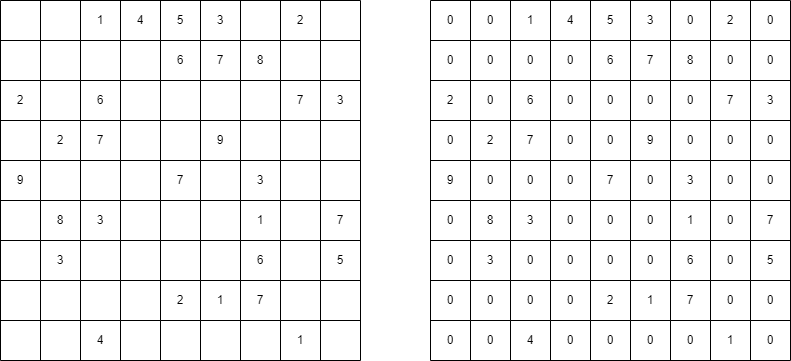
\includegraphics[height=4.5cm, width=10cm]{./Diagrams/representationDiagram}
\end{figure}



\subsection{Puzzle class}
The puzzle class, needs to store the state of the puzzle being solved and the fitness value of the puzzle. The state of the puzzle as previously detailed will be stored in a 2D array of int, the fitness value(s) should be stored in an array of variable size, this allows the puzzle to be set for either type of solver allowing for either single or multi-objective fitness functions. There are two different constructor methods for the puzzle class, a normal constructor and a constructor for copying puzzles. The normal constructor needs the size of the puzzle, the initial puzzle state and number of objectives the fitness function, used to define of the size of the fitness array.\newline \newline The most important methods outside of the setters and getters, are the methods used to find rule violations and empty spaces. The violation finder method, is important for adding rules, where it is used in the repair method as a way to apply the rules of the game to solver and also used as a part of the fitness function for multi-objective. The method is split into several smaller steps, finding each violation for the 3 different rule violations, counting the number of constraint violations each space in the puzzle has and sorting the spaces with violations by number of violations.\newline \newline Finding the constraint violations for the row and column, loops through each space in the row or column and comparing the value to each other space on the board. Counting the grid violations is a similar process, however it has to go through the individual grid, which uses a messier loop. The issues with this way of counting violations, is that it counts each violation twice. The empty spaces algorithm, should return an array of all locations within the puzzle space, that have a 0 value, which is useful for the fitness functions and seeing if the puzzle is complete.

\subsection{Solver Class}

The Solver class is the parent class for the two different types of EA being used in the experiment, so stores their common features, the attributes in the class are, the population which is an ArrayList of puzzle objects, and the initial state of the puzzle which is an array that holds the initial state of the puzzle. The important methods that are used by both solvers, are generating the population, mutation of the individual puzzles, checks for whether the puzzle is complete, a space is part of the initial puzzle and finally a method for loading the initial puzzle from a file.  \newline\newline Generating the intial puzzle, is a simple algorithm, that takes a puzzle, creates the initial state from that puzzle, find the fitness value for the puzzle, then adds mutations of the initial puzzle with updated fitness values, to the population, until the defined size of the population is reached. \newline\newline Mutating a puzzle, displays a different behaviour based on the state of the puzzle. If the puzzle still has empty spaces, it adds a random number between 1 and the puzzle size, to a random empty space in the puzzle. The alternative behaviour is for where all the spaces in the puzzle have been filled, but the puzzle is not yet complete, which only happens to the multi-objective solver, as the repair method for the hybrid solver will always remove values that are violation before mutation happens again. For the alterative behaviour, the mutation changes a random space, that is not in the initial configuration, to a random value between 1 and the puzzle size.\newline\newline The method that checks puzzles completion, looks at every puzzle in the population, if for that puzzle, there are no constraint violations and no empty spaces, meaning the puzzle is full and none of the rules of sudoku have been violated. If a puzzle that meets these conditions is found, the method prints the puzzles state and returns true, if no completed puzzle is found the method returns false. \newline\newline Loading a puzzle from a file is needed in the experiment, the method takes a file path and the puzzle size and simply uses a scanner to read from the file, until there required number of ints are taken for the puzzle size, this does require that the files provided do not use any illegal numbers, outside the range of the puzzle, however given that the this method is only being used specifically for an experiment with files created specifically for that purpose, there is no need to deal with illegal cases. 

\subsection{RepairBasedSolver class}

The RepairBasedSolver class is an implementation of the hybrid repair based EA and is used in the experiment to review the algorithm.\newline\newline The class extends the solver class and only adds 7 unique methods:
\begin{itemize}
	\item getSolution
	\item mutatePopulation
	\item sortPopulation
	\item splitPopulation
	\item repairPuzzle
	\item repairPopulation
	\item updateFitness
\end{itemize}
The getSolution method is the most important method in the class, is an implementation of the EA itself, as detailed in chapter 2.3. Taking a puzzle, the method, generates the population for the algorithm, creates a counter and while loop which checks if the puzzle is completed and the counter has not surpassed the maximum number of generations. Inside the while loop, the counter increases, then the population is repaired, this order changes from figure ?, due to the way the population is generated, as each member is mutated once, meaning many individuals will have have broken the rules, which means without the repair happening before more feasible individuals would be taken out by the selection algorithm. The sort then takes place, with the splitPopulation afterwards before finally mutating and going back to the loop conditions, once the loop has finished the population is cleared and the number of generations taken is returned. \newline\newline The mutation of the population, for each member of the population, creates a copy of the puzzle, mutates and updates the fitness values of both the parent and child puzzle object, then adds the children to the population.\newline\newline The sortPopulation is a method that takes the population and sorts them based on their fitness values. The splitPopulation method acts is the selection algorithm and is rather simple. It removes half the population, by using the sortPopulation all it has to do is remove the front half of the ArrayList. \newline\newline The repairPuzzle method takes the list of violations from the puzzle object, and removes any conflicting space that is not permanent. The repairPopulation method just goes through each member of the population, and loops until the puzzle being looked at is feasible by calling the repairPuzzle method. The updateFitness method takes the roll of the fitness function in this solver class, the fitness calculation is simple, taking the total number of filled spaces as the fitness.

\subsection{Multi-objective class}
The MultiObjectiveSolver class is an implementation of the multi-objective EA and  is used the experiment as one of the two EA being compared.\\\\ It extends the solver class and has 5 methods and a new attribute:
\begin{itemize}
	\item mutatedPopulation
	\item getSolution
	\item mutatePopulation
	\item splitPopulation
	\item compareFitness
	\item updateFitness
\end{itemize}

Mutated population is a field exclusive to the MultiObjectiveSolver class, t is an ArrayList of puzzles which is used to temporarily store puzzles during the mutatePopulation and splitPopulation methods.\\\\ The getSolution method, is the implementation of the EA itself, detailed in chapter 2.4. Taking a puzzle, a population is generated, after this algorithm initiates a counter, used to monitor the number of generations gone through. A while loop, with the conditions to exit the loop being the counter surpassing the maximum number of generations or the puzzle being completed. Inside the loop each time the counter is increased by one. The population then mutates, updates its fitness values and then performs selection on the population. Once one of the exit conditions is satisfied and the loop is exited, the population is cleared, and the number of generations taken is returned. \\\\ The mutatePopulation method, creates a child for each puzzle in the population, these children are added to the mutatedPopulation field, where mutatePuzzle is then used on each of them, and their populations are also updated.\\\\ The splitPopulation method used to represent the selection in the EAs, uses the compareFitness method to compare the fitness of the parent and mutated children puzzle, if the child puzzles fitness values surpasses the parent, it replaces the parent in the main population ArrayList, otherwise the parent stays. Once every member of the population is compared, the mutated population is the then made null.\\\\ The compareFitness function is a helper function used by splitPopulation, it takes two puzzles and compares both of their fitness values, returning true if the first puzzle is greater and false otherwise. The updateFitness method, finds the number of filled spaces and the number of violations that exist.  

\begin{figure}[h]
	\caption{Class diagram for the program}
	\centering
	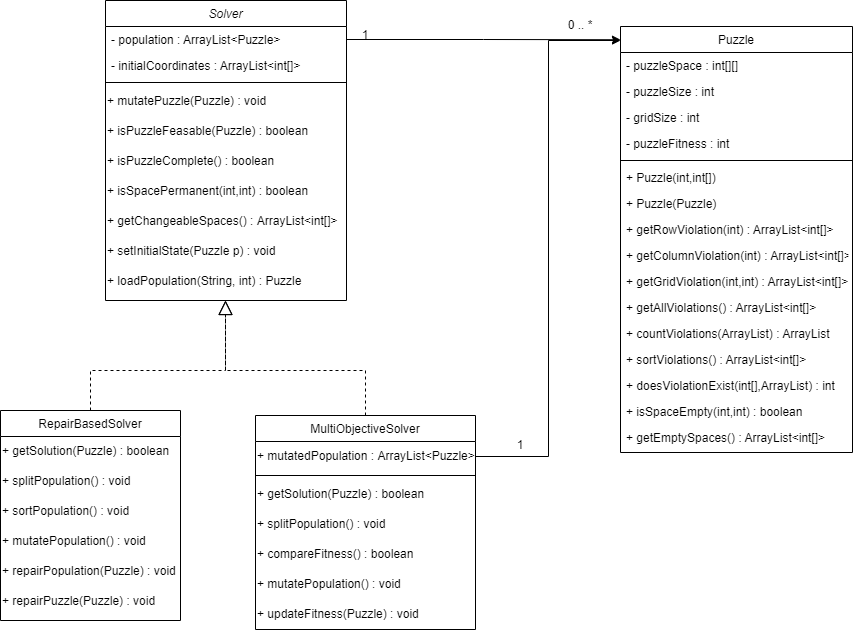
\includegraphics[height=15cm,width=18cm]{./Diagrams/classDiagram}
\end{figure}

\subsection{Experiment program }
The experiments will be done in two steps, the first being collecting data concerning failures and number of generations from the two algorithms performance on a set of sudoku puzzles of different size and difficulty, which will be done in Java. The second step is putting that data in R using scripts and getting greater insights on the results, via graphs and statistical tests.\\ The experiment in Java, will test a solver against 10 puzzle files of some size or difficulty , produce a report of the number of generations and time taken for that attempt. A seperate file will store a report of the average, number of generation(excluding failures), number of failures and time taken. By doing this for all the puzzle sizes and difficulties provided, the data can then be analysed and used for the conclusions. The Java experiment program itself, should for a solver, then for each puzzle, load the puzzle into the solver, and attempt to solve the puzzle 30 times, producing the results detailed earlier and writing them to a file.    

\section{Implementation and testing}

\subsection{Implementation issues}
Throughout the process of implementation, one of the main issues, that hindered further implementation and experimentation, was trying to find the optimal settings and for the evolutionary algorithm. This lead to lots of testing happening trying to find better setting for the algorithm, however this caused further issues, as not only does the randomness of the algorithm make it hard to whether one program is better optimized than another without statistical analysis but also made testing for bugs through manual testing became tedious and hard to repeat, given the same results was unlikely to be produced several times. There was no good way to solve or adapt to these issues, other than manually trying to find the bugs and optimize the algorithm, which slowed down the implementation of the overall program significantly.\\\\ The agile development approach used caused issues, and was not well suited to something like this research project, specifically the use of sprints, meant that not all elements of the program, were planned out before earlier part integral to the structure, had been implemented. This caused issues in two different ways, some of the earlier parts had to be completely overhauled which wasted project time, whilst others were just kept making the algorithms less effective or producing more bugs later on. \\\\The issue of randomness, was particularly bad for the hybrid method, as it was already quite inconsistent, this made testing to see whether any adjustments made to the algorithm, generally did not show results without large amounts of testing, especially for the 9x9 sudokus, which take significantly longer to run than the 4x4s. The other issue was making small adjustments to program for improvements was hard to track on the 4x4 puzzle, as the number of generations was generally so small, that it couldn't be improved much, so the only changes that would show is when the number of generations greatly increases. \\\\For the multi-objective EA implementation, there was a misconception on how to use and compare the fitness values of two different puzzles, which took several weeks to realise that the wrong approach was being used. A similar problem happened for the overall design of the selection and mutation functions which were being applied in a inefficient manner, however when the repair class was changed to apply with the new method, it could no longer produce results for the puzzles, so these changes were reverted for the repair based solver only, meaning that it is less effective than it could be.\\\\
Several simple issues were made during the experiment phase, specifically surrounding writing the results to files, with results being incorrectly recorded, overwritten and deleted, which lead to experiments having to be run several times. This admittedly could have been avoided by properly testing out the experiment code on a smaller set of data using test file locations.
\subsection{Testing }
There was no define approach to how the testing was created, some of the tests were created after the methods as a way to check their behaviour, and some tests were done in the test driven development style, where tests were made first and methods were created to pass the tests. Due to the nature of the project, the testing itself, only really has to cover finding errors and checking method behaviour, given that there is no user or for the system. The two different types of tests used in the project have been automatic and manual testing.
\subsubsection{Automatic testing}
The automatic testing, uses the 3rd party library JUnit and covers most of the important methods in the Puzzle, Solver, RepairBasedSolver and MultiObjectiveSolver classes. It was also used to do the initial tests for the getSolution methods, which in this program is the integration tests given that the two solver classes getSolution use most of the components.  
\subsubsection{Manual testing}
The manual testing for the project was done, when behaviours in the outputs of the different solvers were found that were not intentional. The testing was mostly trying to recreate the conditions of the bug, however difficult it was given the randomness and using the breakpoints and debugger in the IntelliJ IDE to identify what was going wrong.


\end{document}